\documentclass[11pt,a4paper]{article}
\usepackage[utf8]{inputenc}
\usepackage[T1]{fontenc}
\usepackage{lmodern}
\usepackage{amsmath}
\usepackage{amsfonts}
\usepackage{amssymb}
\usepackage{graphicx}
\usepackage{hyperref}
\usepackage{xcolor}
\usepackage{listings}
\usepackage{tikz}
\usetikzlibrary{positioning}
\usepackage{float}
\usepackage{enumitem}
\usepackage{booktabs}
\usepackage{caption}
\usepackage{subcaption}
\usepackage{fancyhdr}
\usepackage{geometry}
\usepackage{titlesec}

\geometry{a4paper, margin=1in}

\hypersetup{
    colorlinks=true,
    linkcolor=blue,
    filecolor=magenta,
    urlcolor=cyan,
    pdftitle={DarkSwap: A Decentralized Exchange for Bitcoin, Runes, and Alkanes},
    pdfauthor={DarkSwap Team},
    pdfsubject={Decentralized Exchange},
    pdfkeywords={Bitcoin, DEX, P2P, Runes, Alkanes}
}

\title{
    \vspace{2cm}
    \Huge{\textbf{DarkSwap}}\\
    \vspace{0.5cm}
    \Large{A Decentralized Exchange for Bitcoin, Runes, and Alkanes}\\
    \vspace{0.5cm}
    \large{Whitepaper v1.0}\\
    \vspace{2cm}
}

\author{DarkSwap Team}
\date{\today}

\begin{document}

\maketitle
\thispagestyle{empty}
\newpage

\tableofcontents
\newpage

\section*{Abstract}
\addcontentsline{toc}{section}{Abstract}

DarkSwap is a decentralized exchange (DEX) platform designed specifically for Bitcoin, runes, and alkanes. Unlike traditional centralized exchanges, DarkSwap enables direct peer-to-peer trading without intermediaries, enhancing security, privacy, and user control. This whitepaper presents the architecture, technical components, and security model of DarkSwap, highlighting its innovative approach to decentralized trading on Bitcoin. By leveraging advanced peer-to-peer networking, WebRTC technology, and end-to-end encryption, DarkSwap provides a secure, private, and user-friendly platform for cryptocurrency trading without the risks associated with centralized exchanges.

\newpage

\section{Introduction}

The cryptocurrency ecosystem has seen significant growth in decentralized finance (DeFi) applications, particularly decentralized exchanges. However, most existing DEX solutions focus on Ethereum and other smart contract platforms, with limited support for Bitcoin—the largest and most established cryptocurrency. Additionally, the emergence of runes and alkanes as new asset types on Bitcoin has created a need for specialized trading platforms.

DarkSwap addresses this gap by providing a decentralized exchange specifically designed for Bitcoin, runes, and alkanes. By enabling direct peer-to-peer trading without centralized intermediaries, DarkSwap eliminates the risks associated with centralized exchanges, such as hacks, asset freezes, and privacy concerns.

The key innovations of DarkSwap include:

\begin{itemize}
    \item A pure peer-to-peer architecture with no central server or authority
    \item Advanced WebRTC-based networking for browser and desktop compatibility
    \item Circuit relay technology for reliable NAT traversal
    \item End-to-end encryption for secure communications
    \item Comprehensive authentication and authorization systems
    \item Efficient connection pooling and relay discovery mechanisms
    \item Cross-platform support across desktop and web environments
\end{itemize}

This whitepaper provides a detailed overview of DarkSwap's architecture, components, security model, and roadmap, demonstrating how it addresses the challenges of decentralized trading on Bitcoin.

\section{Background and Problem Statement}

\subsection{Centralized Exchange Risks}

Centralized cryptocurrency exchanges have been plagued by numerous issues:

\begin{itemize}
    \item \textbf{Security Breaches}: Numerous high-profile hacks resulting in billions of dollars in losses
    \item \textbf{Asset Control}: Users must surrender control of their private keys
    \item \textbf{Counterparty Risk}: Exposure to exchange insolvency or mismanagement
    \item \textbf{Privacy Concerns}: KYC requirements and transaction monitoring
    \item \textbf{Censorship}: Ability to freeze assets or block transactions
    \item \textbf{Regulatory Uncertainty}: Vulnerability to changing regulations
\end{itemize}

\subsection{Limitations of Existing DEX Solutions}

While decentralized exchanges address many of these issues, they come with their own limitations:

\begin{itemize}
    \item \textbf{Limited Bitcoin Support}: Most DEXs focus on Ethereum and other smart contract platforms
    \item \textbf{Complex User Experience}: Technical barriers for average users
    \item \textbf{Connectivity Issues}: P2P systems often struggle with NAT traversal
    \item \textbf{Limited Asset Support}: Few platforms support runes and alkanes
    \item \textbf{Performance Constraints}: Slower execution compared to centralized alternatives
    \item \textbf{Liquidity Challenges}: Fragmented liquidity across platforms
\end{itemize}

\subsection{The Need for Bitcoin-Native DEX}

Bitcoin's ecosystem has evolved with the introduction of runes and alkanes, creating new opportunities for asset creation and trading. However, these innovations lack dedicated trading infrastructure that preserves Bitcoin's core values of decentralization, security, and user sovereignty.

A Bitcoin-native DEX must address several unique challenges:

\begin{itemize}
    \item Operating without smart contracts that are common on other platforms
    \item Ensuring secure peer-to-peer trading of Bitcoin and Bitcoin-based assets
    \item Providing reliable networking across diverse network conditions
    \item Maintaining privacy while enabling efficient trading
    \item Supporting cross-platform usage, including browsers
\end{itemize}

DarkSwap is designed specifically to address these challenges, providing a secure, private, and user-friendly platform for trading Bitcoin, runes, and alkanes without centralized intermediaries.

\section{Solution Overview}

DarkSwap is a comprehensive decentralized exchange platform built on a pure peer-to-peer architecture. It enables direct trading between users without relying on centralized servers or authorities for matching or executing trades.

\subsection{Core Principles}

DarkSwap is built on the following core principles:

\begin{itemize}
    \item \textbf{Decentralization}: No central authority controls the platform or user funds
    \item \textbf{Security}: Strong encryption, authentication, and authorization mechanisms
    \item \textbf{Privacy}: Minimal data collection and end-to-end encrypted communications
    \item \textbf{User Control}: Users maintain control of their private keys and funds
    \item \textbf{Usability}: Intuitive interfaces that abstract technical complexity
    \item \textbf{Cross-Platform}: Support for both desktop and web environments
\end{itemize}

\subsection{Key Components}

DarkSwap consists of several key components:

\begin{itemize}
    \item \textbf{DarkSwap SDK}: Core functionality and APIs
    \item \textbf{DarkSwap CLI}: Command-line interface for interacting with the platform
    \item \textbf{DarkSwap Daemon}: Background service for handling ongoing operations
    \item \textbf{DarkSwap P2P}: Peer-to-peer networking infrastructure
    \item \textbf{Web Interface}: Browser-based user interface
\end{itemize}

\subsection{Trading Flow}

The typical trading flow in DarkSwap follows these steps:

\begin{enumerate}
    \item User creates or imports a wallet
    \item User connects to the P2P network
    \item User browses the distributed order book
    \item User places a buy or sell order
    \item Order is broadcast to the network
    \item When a matching order is found, users are connected directly
    \item Trade is executed peer-to-peer with atomic swap guarantees
    \item Transaction is broadcast to the Bitcoin network
    \item Order book is updated to reflect the completed trade
\end{enumerate}

This flow ensures that users maintain control of their funds throughout the trading process, with no centralized intermediary holding custody at any point.

\section{Technical Architecture}

DarkSwap employs a modular architecture with clear separation of concerns, allowing for independent development, testing, and deployment of components.

\subsection{System Architecture}

\begin{figure}[H]
    \centering
    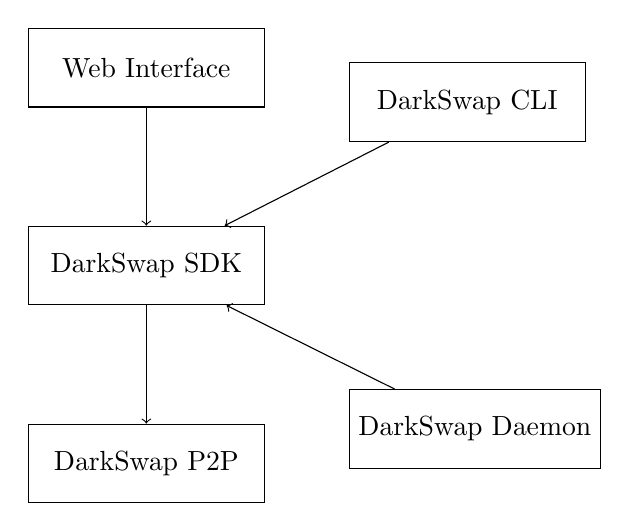
\begin{tikzpicture}[node distance=1.5cm]
        \node (sdk) [rectangle, draw, minimum width=3cm, minimum height=1cm] {DarkSwap SDK};
        \node (cli) [rectangle, draw, minimum width=3cm, minimum height=1cm, above right=of sdk] {DarkSwap CLI};
        \node (daemon) [rectangle, draw, minimum width=3cm, minimum height=1cm, below right=of sdk] {DarkSwap Daemon};
        \node (p2p) [rectangle, draw, minimum width=3cm, minimum height=1cm, below=of sdk] {DarkSwap P2P};
        \node (web) [rectangle, draw, minimum width=3cm, minimum height=1cm, above=of sdk] {Web Interface};
        
        \draw[->] (cli) -- (sdk);
        \draw[->] (daemon) -- (sdk);
        \draw[->] (web) -- (sdk);
        \draw[->] (sdk) -- (p2p);
    \end{tikzpicture}
    \caption{DarkSwap System Architecture}
\end{figure}

\subsection{Component Details}

\subsubsection{DarkSwap SDK}

The SDK provides the core functionality and APIs, including:

\begin{itemize}
    \item Wallet management
    \item Order book handling
    \item Trade execution
    \item Type definitions
\end{itemize}

It is implemented in Rust for performance, security, and cross-platform compatibility, with WebAssembly bindings for browser environments.

\subsubsection{DarkSwap P2P}

The P2P networking layer is a critical component, providing:

\begin{itemize}
    \item WebRTC transport for browser compatibility
    \item Circuit relay for NAT traversal
    \item Connection pooling for efficient connection management
    \item Relay discovery and ranking
    \item Authentication and authorization
    \item End-to-end encryption
    \item Metrics and monitoring
\end{itemize}

This component enables reliable peer-to-peer communication across diverse network conditions, including browsers and devices behind NATs.

\subsubsection{DarkSwap CLI}

The command-line interface provides:

\begin{itemize}
    \item User commands for trading and wallet management
    \item Configuration management
    \item Status reporting
    \item Automation capabilities
\end{itemize}

\subsubsection{DarkSwap Daemon}

The background service handles:

\begin{itemize}
    \item Long-running processes
    \item Event handling
    \item System integration
    \item Network maintenance
\end{itemize}

\subsubsection{Web Interface}

The browser-based interface provides:

\begin{itemize}
    \item React components for user interaction
    \item WebRTC integration for P2P communication
    \item Responsive design for various devices
    \item WebAssembly integration with the SDK
\end{itemize}

\subsection{Technology Stack}

DarkSwap leverages a modern technology stack:

\begin{itemize}
    \item \textbf{Programming Languages}:
    \begin{itemize}
        \item Rust for core components, SDK, daemon, and CLI
        \item TypeScript for web interface and browser integration
        \item WebAssembly (WASM) for running Rust code in browsers
    \end{itemize}
    
    \item \textbf{Core Libraries}:
    \begin{itemize}
        \item libp2p for peer-to-peer networking
        \item tokio for asynchronous runtime
        \item ring for cryptographic operations
        \item bdk (Bitcoin Dev Kit) for Bitcoin wallet functionality
        \item React for web UI
        \item WebRTC for browser-based P2P communication
    \end{itemize}
\end{itemize}

\section{Key Features and Components}

\subsection{P2P Networking}

DarkSwap's P2P networking layer is built on several innovative technologies:

\subsubsection{WebRTC Transport}

WebRTC enables direct browser-to-browser communication, allowing DarkSwap to work in web environments without centralized servers. Key features include:

\begin{itemize}
    \item Direct peer connections using WebRTC data channels
    \item Signaling server for initial connection establishment
    \item ICE candidate exchange for NAT traversal
    \item Efficient binary data transfer
\end{itemize}

\subsubsection{Circuit Relay}

To overcome NAT traversal challenges, DarkSwap implements circuit relay:

\begin{itemize}
    \item Relay nodes facilitate connections between peers behind NATs
    \item Relay discovery mechanism finds and ranks available relays
    \item Connection establishment through optimal relay paths
    \item Fallback mechanisms for challenging network conditions
\end{itemize}

\subsubsection{Connection Pooling}

For efficient connection management, DarkSwap implements connection pooling:

\begin{itemize}
    \item Reuse of existing connections to reduce overhead
    \item Connection lifecycle management
    \item Automatic pruning of expired connections
    \item Performance optimization for high-traffic scenarios
\end{itemize}

\subsection{Security Features}

\subsubsection{Authentication and Authorization}

DarkSwap implements a comprehensive authentication system:

\begin{itemize}
    \item Multiple authentication methods (shared key, challenge-response, public key)
    \item Authorization levels for different operations
    \item Trusted and banned peer management
    \item Token-based authentication with automatic expiration
\end{itemize}

\subsubsection{End-to-End Encryption}

All communications are protected with strong encryption:

\begin{itemize}
    \item Multiple encryption algorithms (AES-GCM-256, ChaCha20-Poly1305)
    \item X25519 key exchange for secure key agreement
    \item Forward secrecy with ephemeral keys
    \item Key rotation and automatic key expiration
\end{itemize}

\subsection{Wallet Integration}

DarkSwap supports multiple wallet implementations:

\begin{itemize}
    \item Simple wallet for basic functionality
    \item BDK wallet for advanced Bitcoin operations
    \item Support for Bitcoin, runes, and alkanes
    \item Secure key management
    \item Transaction creation and signing
\end{itemize}

\subsection{Order Book Management}

The distributed order book system provides:

\begin{itemize}
    \item Order creation and validation
    \item Order storage and retrieval
    \item Order matching algorithms
    \item Order distribution across the network
\end{itemize}

\subsection{Trade Execution}

The trade execution system ensures:

\begin{itemize}
    \item Secure peer-to-peer trade protocol
    \item Transaction validation
    \item Atomic swap guarantees
    \item Error handling for failed trades
\end{itemize}

\subsection{Monitoring and Metrics}

For system health and performance tracking:

\begin{itemize}
    \item Comprehensive metrics collection
    \item Prometheus integration
    \item Grafana dashboards
    \item Alerting system
\end{itemize}

\section{Security Model}

DarkSwap employs a defense-in-depth security approach with multiple layers of protection.

\subsection{Threat Model}

The security model addresses several threat vectors:

\begin{itemize}
    \item \textbf{Network Attacks}: Man-in-the-middle, eavesdropping, replay attacks
    \item \textbf{Identity Spoofing}: Impersonation of peers or relays
    \item \textbf{Denial of Service}: Resource exhaustion attacks
    \item \textbf{Trade Manipulation}: Attempts to manipulate order matching or execution
    \item \textbf{Wallet Compromise}: Unauthorized access to wallet keys
\end{itemize}

\subsection{Security Layers}

\subsubsection{Network Security}

\begin{itemize}
    \item End-to-end encryption of all communications
    \item Authenticated connections between peers
    \item Secure relay selection and connection
    \item Protection against replay and man-in-the-middle attacks
\end{itemize}

\subsubsection{Authentication Security}

\begin{itemize}
    \item Multiple authentication methods for flexibility and strength
    \item Challenge-response protocols for secure verification
    \item Token-based authentication with automatic expiration
    \item Authorization levels for access control
\end{itemize}

\subsubsection{Wallet Security}

\begin{itemize}
    \item Local key storage with no server uploads
    \item Optional encryption of wallet files
    \item Minimal exposure of private keys
    \item Transaction verification before signing
\end{itemize}

\subsubsection{Trade Security}

\begin{itemize}
    \item Atomic swap protocols for trade execution
    \item Transaction validation before acceptance
    \item Protection against double-spending attempts
    \item Timeout mechanisms for incomplete trades
\end{itemize}

\subsection{Security Principles}

DarkSwap follows key security principles:

\begin{itemize}
    \item \textbf{Defense in Depth}: Multiple security layers
    \item \textbf{Principle of Least Privilege}: Minimal access rights
    \item \textbf{Forward Secrecy}: Protection of past communications
    \item \textbf{Zero Trust}: Verification of all peers and operations
    \item \textbf{Fail Secure}: Default to secure state on failure
\end{itemize}

\section{Use Cases}

DarkSwap addresses several key use cases for different user types.

\subsection{Bitcoin Trading}

\begin{itemize}
    \item Secure peer-to-peer Bitcoin trading without intermediaries
    \item Private transactions without KYC requirements
    \item Self-custody throughout the trading process
    \item Protection from exchange hacks and freezes
\end{itemize}

\subsection{Runes and Alkanes Trading}

\begin{itemize}
    \item Specialized support for these Bitcoin-based assets
    \item Efficient discovery of trading partners
    \item Secure execution of trades
    \item Integration with Bitcoin wallets supporting these assets
\end{itemize}

\subsection{Privacy-Focused Trading}

\begin{itemize}
    \item End-to-end encrypted communications
    \item No central server monitoring transactions
    \item Minimal data collection and storage
    \item Protection from surveillance and tracking
\end{itemize}

\subsection{Cross-Platform Trading}

\begin{itemize}
    \item Consistent experience across desktop and web
    \item Browser-based trading without downloads
    \item Desktop application for enhanced performance
    \item Interoperability between platforms
\end{itemize}

\subsection{Developer Integration}

\begin{itemize}
    \item SDK for building custom applications
    \item API access for integration with other services
    \item Extensible architecture for custom features
    \item Documentation and examples for developers
\end{itemize}

\section{Roadmap}

DarkSwap development follows a phased approach:

\subsection{Phase 1: Foundation (Completed)}

\begin{itemize}
    \item Core P2P networking infrastructure
    \item Basic wallet integration
    \item Simple order book functionality
    \item Command-line interface
\end{itemize}

\subsection{Phase 2: Enhancement (Completed)}

\begin{itemize}
    \item Advanced P2P capabilities
    \item Improved wallet functionality
    \item Enhanced order book and trade execution
    \item Initial web interface
\end{itemize}

\subsection{Phase 3: Production Readiness (Current)}

\begin{itemize}
    \item Security hardening (authentication, encryption)
    \item Performance optimization
    \item Comprehensive testing
    \item Monitoring and metrics
    \item User experience improvements
\end{itemize}

\subsection{Phase 4: Public Launch (Planned)}

\begin{itemize}
    \item Public beta release
    \item Community building
    \item Documentation and tutorials
    \item Bug fixes and stability improvements
\end{itemize}

\subsection{Phase 5: Ecosystem Growth (Future)}

\begin{itemize}
    \item API enhancements for developers
    \item Additional asset support
    \item Advanced trading features
    \item Mobile applications
    \item Integration with other Bitcoin projects
\end{itemize}

\section{Conclusion}

DarkSwap represents a significant advancement in decentralized exchange technology for Bitcoin, runes, and alkanes. By combining innovative peer-to-peer networking, strong security features, and user-friendly interfaces, DarkSwap addresses the limitations of both centralized exchanges and existing DEX solutions.

The platform's modular architecture, advanced P2P capabilities, and comprehensive security model provide a solid foundation for secure, private, and efficient trading without centralized intermediaries. As DarkSwap progresses through its roadmap, it aims to become the leading decentralized exchange for Bitcoin and Bitcoin-based assets, empowering users with true financial sovereignty.

By prioritizing security, privacy, and user control, DarkSwap aligns with the core principles of Bitcoin itself, offering a trading platform that preserves these values while providing the functionality and user experience expected in modern financial applications.

\section{References}

\begin{enumerate}
    \item Bitcoin: A Peer-to-Peer Electronic Cash System. Satoshi Nakamoto, 2008.
    \item WebRTC 1.0: Real-Time Communication Between Browsers. W3C, 2021.
    \item libp2p: A Modular Network Stack. Protocol Labs, 2022.
    \item Circuit Relay Protocol. libp2p Specifications, 2023.
    \item Bitcoin Development Kit (BDK) Documentation, 2024.
    \item Atomic Swap Protocol for Cryptocurrencies, 2020.
    \item Runes: A Bitcoin-Native Asset Protocol, 2023.
    \item Alkanes: Extended Asset Protocol for Bitcoin, 2024.
\end{enumerate}

\end{document}